\documentclass{article}
\usepackage[UTF8]{ctex}
\usepackage{tikz}
\usepackage{caption}
\usepackage{amsmath}
\usepackage[total={7in,10in}]{geometry}

\usetikzlibrary{decorations.markings}

\begin{document}

\section*{试题}

\begin{enumerate}

\item
人们看到的彩虹是在空气中的水珠内被反射过的光.
定义 $k$ 级虹为在空气中的水珠内经历过 $k-1$ 次反射的光产生的彩虹.
在中国古代, 人们将二级虹称为虹, 而将三级虹称为霓.

在春分日的正午于北纬 $\alpha$ 处下了一场雨.
雨后空气中均匀且密集地分布着球形小水珠, 于是此地的观察者在天球上观察到了彩虹.

地平坐标系是一种天球坐标系统, 以观测者所在地为中心点, 所在地的地平线为基础平面.
在地平坐标系中, 用高度角 (地平纬度) $\theta$ 和方位角 (地平经度) $\varphi$ 来指定天球上的点,
其中方位角以正北开始向东测量.

\begin{enumerate}

	\item
	某色光在水中的折射率为 $n$.
	求天球上 $k$ 级虹中该颜色的曲线在地平坐标系中的方程.

	\item
	可见光在水中的折射率的范围为 $\left[n,n+\Delta n\right]$, 其中 $\Delta n\ll n$.
	求 $k$ 级虹在天顶 (天球的上半部分) 上占据的立体角, 保留到关于 $\Delta n$ 的一阶小量.

	\item
	考虑到在观察者眼中, 太阳绕地球以角速度 $\omega$ 自东向西旋转,
	求 $k$ 级虹的在水中折射率为 $n$ 的颜色的曲线上的在天球上具有最大高度角的点的方位角的变化率 (注意正负号).
\end{enumerate}

\end{enumerate}

\newpage
\section*{参考答案}

\begin{enumerate}

\item
\begin{enumerate}

	\item
	考虑一条被水珠折射的光线.
	因为球表面的法线过球心, 所以光线所在平面过球心.
	光路如图 \ref{fig:水珠光路图} 所示.

	\begin{figure}[h!]
		\centering
		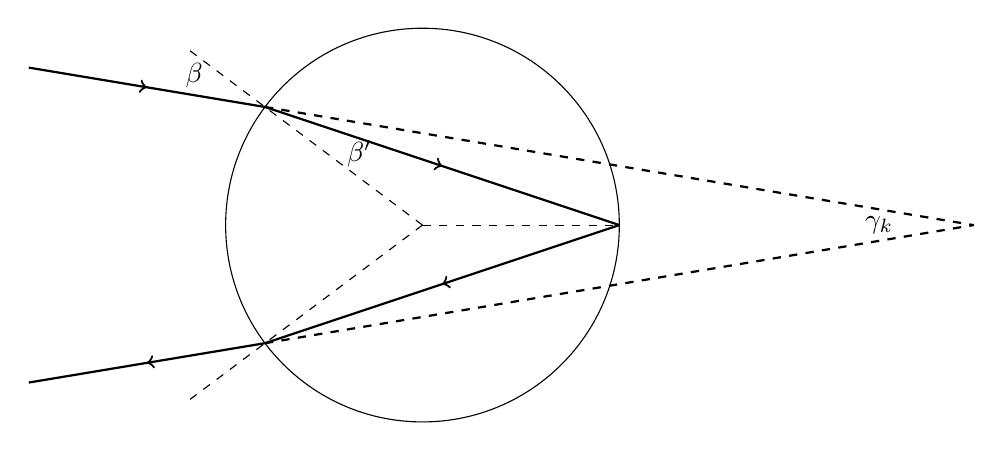
\begin{tikzpicture}
			\draw (0, 0) circle (2.5);
			\begin{scope}[thick,decoration={
					markings,
					mark=at position 0.5 with {\arrow{>}}}
					]
				\draw[postaction={decorate}] (-5,2) -- (-2,1.5);
				\draw[postaction={decorate}] (-2,1.5) -- (2.5,0);
				\draw[postaction={decorate}] (2.5,0) -- (-2,-1.5);
				\draw[postaction={decorate}] (-2,-1.5) -- (-5,-2);
			\end{scope}
			\draw[thick,dashed] (-2,1.5) -- (7,0);
			\draw[thick,dashed] (-2,-1.5) -- (7,0);
			\draw[dashed] (0,0) -- (-3,2.25);
			\draw[dashed] (0,0) -- (-3,-2.25);
			\draw[dashed] (0,0) -- (2.5,0);
			\node at (-2.9,1.9) {$\beta$};
			\node at (-0.8,0.9) {$\beta'$};
			\node at (5.8,0) {$\gamma_k$};
		\end{tikzpicture}
		\caption{}
		\label{fig:水珠光路图}
	\end{figure}

	设该光线以入射角 $\beta$ 射入水珠, 从而折射角
	\begin{equation}
		\beta'=\arcsin\frac{\sin\beta}n.
	\end{equation}
	每次折射会造成偏转角 $\beta-\beta'$, 每次在水珠内反射会造成偏转角 $\pi-2\beta'$.
	总共经历了 $2$ 次折射和 $k-1$ 次反射, 所以总偏转角
	\begin{equation}
		\pi-\gamma_k=2\left(\beta-\beta'\right)+\left(k-1\right)\left(\pi-2\beta'\right),
	\end{equation}
	即入射光线和出射光线的夹角
	\begin{equation}
		\gamma_k=\left(2-k\right)\pi-2\beta+2k\arcsin\frac{\sin\beta}n.
		\label{eq:gamma_k}
	\end{equation}

	设入射光强按 $\beta$ 的分布为 $I\left(\beta\right)\mathrm d\beta$.
	显然 $I\left(\beta\right)$ 没有奇点.
	但是, 出射光强按 $\gamma_k$ 的分布 $I\left(\beta\right)\frac{\partial\beta}{\partial\gamma_k}\mathrm d\gamma_k$ 可能存在奇点 $\beta=\beta_k$,
	即
	\begin{equation}
		\left.\frac{\partial\gamma_k}{\partial\beta}\right|_{\beta=\beta_k}=-2+2k\frac{\frac{\cos\beta_k}n}{\sqrt{1-\frac{\sin^2\beta_k}{n^2}}}=0.
	\end{equation}
	解得
	\begin{equation}
		\label{eq:beta_k}
		\beta_k=\arcsin\sqrt{\frac{k^2-n^2}{k^2-1}}.
	\end{equation}
	将式 \ref{eq:beta_k} 代入式 \ref{eq:gamma_k} 可得
	\begin{equation}
		\gamma_k=\left(2-k\right)\pi-2\arcsin\sqrt{\frac{k^2-n^2}{k^2-1}}+2k\arcsin\left(\frac1n\sqrt{\frac{k^2-n^2}{k^2-1}}\right).
		\label{eq:完整的gamma_k}
	\end{equation}

	在 $\beta=\beta_k$ 处光强发散至无穷大, 因此天球上呈现的曲线就来自于以这一角度入射的光线.

	\begin{figure}[h!]
		\centering
		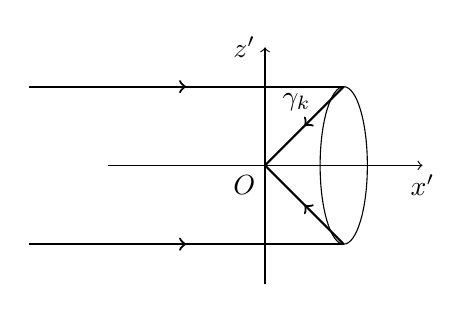
\begin{tikzpicture}
			\begin{scope}[thick,decoration={
					markings,
					mark=at position 0.5 with {\arrow{>}}}
					]
				\draw[postaction={decorate}] (-3,1) -- (1,1);
				\draw[postaction={decorate}] (1,1) -- (0,0);
				\draw[postaction={decorate}] (-3,-1) -- (1,-1);
				\draw[postaction={decorate}] (1,-1) -- (0,0);
			\end{scope}
			\draw (1,0) ellipse (0.3 and 1);
			\node[anchor=north east] at (0,0) {$O$};
			\draw[->] (-2,0) -- (2,0) node [below] {$x'$};
			\draw[->] (0,-1.5) -- (0,1.5) node [left] {$z'$};
			\node at (0.4,0.8) {$\gamma_k$};
		\end{tikzpicture}
		\caption{}
		\label{fig:总光路图}
	\end{figure}

	即, 若正好背对着太阳看, $k$ 级虹为视角为 $2\gamma_k$ 的圆, 如图 \ref{fig:总光路图} 所示.
	若以阳光传播的方向为 $x'$ 轴, 以观察者的位置为原点, 则 $k$ 级虹的曲线方程为
	\begin{equation}
		\begin{cases}
			y'^2+z'^2=\sin^2\gamma_k,\\
			x'=\cos\gamma_k.
		\end{cases}
		\label{eq:换系前}
	\end{equation}

	以向北为 $x$ 轴, 向东为 $y$ 轴 (左手系).
	由如图 \ref{fig:换系} 所示的几何关系, 可得 $Oxyz$ 系与 $Ox'y'z'$ 系间的变换关系
	\begin{equation}
		\left[\begin{matrix}x'\\y'\\z'\end{matrix}\right]=
		\left[\begin{matrix}\sin\alpha & 0 & -\cos\alpha \\ 0 & 1 & 0 \\ \cos\alpha & 0 & \sin\alpha\end{matrix}\right]
		\left[\begin{matrix}x\\y\\z\end{matrix}\right].
		\label{eq:换系}
	\end{equation}

	\begin{figure}[h!]
		\centering
		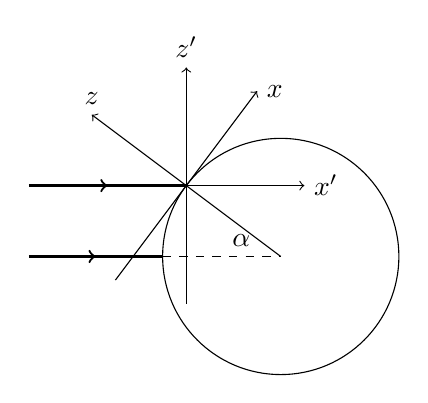
\begin{tikzpicture}
			\draw[->] (1.2,-0.9) circle (1.5);
			\draw[->] (-1.5,0) -- (1.5,0) node [right] {$x'$};
			\draw[->] (0,-1.5) -- (0,1.5) node [above] {$z'$};
			\draw[->] (-0.9,-1.2) -- (0.9,1.2) node [right] {$x$};
			\draw[->] (1.2,-0.9) -- (-1.2,0.9) node [above] {$z$};
			\draw[dashed] (-0.3,-0.9) -- (1.2,-0.9);
			\begin{scope}[thick,decoration={
					markings,
					mark=at position 0.5 with {\arrow{>}}}
					]
				\draw[postaction={decorate}] (-2,0) -- (0,0);
				\draw[postaction={decorate}] (-2,-0.9) -- (-0.3,-0.9);
			\end{scope}
			\node at (0.7,-0.7) {$\alpha$};
		\end{tikzpicture}
		\caption{}
		\label{fig:换系}
	\end{figure}

	将式 \ref{eq:换系} 代入式 \ref{eq:换系前} 可得新的曲线方程
	\begin{equation}
		\begin{cases}
			y^2+\left(x\cos\alpha+z\sin\alpha\right)^2=\sin^2\gamma_k,\\
			x\sin\alpha-z\cos\alpha=\cos\gamma_k.
		\end{cases}
		\label{eq:换系后}
	\end{equation}

	考虑到地平坐标系的定义, 我们有变换
	\begin{equation}
		\left[\begin{matrix}x\\y\\z\end{matrix}\right]=
		\left[\begin{matrix}\cos\theta\cos\varphi \\ \cos\theta\sin\varphi \\ \sin\theta\end{matrix}\right].
		\label{eq:地平坐标系}
	\end{equation}
	将式 \ref{eq:地平坐标系} 代入式 \ref{eq:换系后} 可得地平坐标系中 $k$ 级虹的曲线方程
	\begin{equation}
		\begin{cases}
			\cos^2\theta\sin^2\varphi+\left(\cos\theta\cos\varphi\cos\alpha+\sin\theta\sin\alpha\right)^2=\sin^2\gamma_k,\\
			\cos\theta\cos\varphi\sin\alpha-\sin\theta\cos\alpha=\cos\gamma_k.
		\end{cases}
		\label{eq:地平坐标系冗余曲线方程}
	\end{equation}
	但是注意到式 \ref{eq:地平坐标系冗余曲线方程} 中的两式可以相互推出 (这源于球坐标自带球面约束而导致的坐标数量的减少), 实际上可以简化为一个式子
	\begin{equation}
		\cos\theta\cos\varphi\sin\alpha-\sin\theta\cos\alpha=\cos\gamma_k.
		\label{eq:地平坐标系曲线方程}
	\end{equation}

	式 \ref{eq:地平坐标系曲线方程} 和式 \ref{eq:完整的gamma_k} 给出了答案.

	\item
	需要求出式 \ref{eq:地平坐标系曲线方程} 所描述的曲线上使得 $\theta>0$ (即在天顶上) 的部分 (圆弧) 的长度占整条曲线 (圆) 的比例 $r$.
	为此, 将
	\begin{equation}
		\theta=0
		\label{eq:地平线}
	\end{equation}
	代入式 \ref{eq:地平坐标系曲线方程}, 得
	\begin{equation}
		\cos\varphi=\frac{\cos\gamma_k}{\sin\alpha}.
		\label{eq:地平线上的phi满足的方程}
	\end{equation}

	\begin{enumerate}

		\item
		对于 $\left|\sin\alpha\right|<\left|\cos\gamma_k\right|$, 式 \ref{eq:地平线上的phi满足的方程} 无解.
		从而 $k$ 级虹与地平线没有交点, 即人们能看到完整的圆形虹 ($r=1$)或完全看不到虹 ($r=0$).
		经过简单分析可得, 这种情形下, 对于 $\cos\gamma_k>0$, 有 $r=0$; 对于 $\cos\gamma_k<0$, 有 $r=1$.

		\item
		对于 $\left|\sin\alpha\right|>\left|\cos\gamma_k\right|$, 式 \ref{eq:地平线上的phi满足的方程} 的解 (在模 $2\pi$ 下) 为
		\begin{equation}
			\varphi=\pm\arccos\frac{\cos\gamma_k}{\sin\alpha}.
			\label{eq:地平线上的phi}
		\end{equation}
		将式 \ref{eq:地平线} 和式 \ref{eq:地平线上的phi} 代入式 \ref{eq:地平坐标系} 可得 $k$ 级虹与地平线的交点为
		$\left(\frac{\cos\gamma_k}{\sin\alpha},\pm\sqrt{1-\frac{\cos^2\gamma_k}{\sin^2\alpha}},0\right)$.
		即, $k$ 级虹被地平线所截弦所对的圆心角为
		\begin{equation}
			\psi=2\arcsin\frac{\sqrt{1-\frac{\cos^2\gamma_k}{\sin^2\alpha}}}{\left|\sin\gamma_k\right|}.
		\end{equation}
		经过简单分析可得, 在这种情况下, 对于 $\cos\gamma_k>0$, 有 $r=\frac\psi{2\pi}$; 对于 $\cos\gamma_k<0$, 有 $r=1-\frac\psi{2\pi}$.

	\end{enumerate}

	注意到 $\Delta n$ 为小量, 故由式 \ref{eq:完整的gamma_k} 有
	\begin{equation}
		\Delta\gamma_k=\frac{\partial\gamma_k}{\partial n}\Delta n=-\frac{2\Delta n}n\sqrt{\frac{k^2-n^2}{n^2-1}}.
		\label{eq:delta gamma_k}
	\end{equation}
	从而利用式 \ref{eq:delta gamma_k} 易得答案
	\begin{equation}
		\Omega=r\cdot2\pi\left|\sin\gamma_k\cdot\Delta\gamma_k\right|=4\pi r\left|\sin\gamma_k\right|\frac{\Delta n}n\sqrt{\frac{k^2-n^2}{n^2-1}},
	\end{equation}
	其中
	\begin{equation}
		r=
		\begin{cases}
			0, & \left|\sin\alpha\right|<\left|\cos\gamma_k\right|,\cos\gamma_k>0\\
			1, & \left|\sin\alpha\right|<\left|\cos\gamma_k\right|,\cos\gamma_k<0\\
			\frac1\pi\arcsin\frac{\sqrt{1-\frac{\cos^2\gamma_k}{\sin^2\alpha}}}{\left|\sin\gamma_k\right|}, & \left|\sin\alpha\right|>\left|\cos\gamma_k\right|,\cos\gamma_k>0\\
			1-\frac1\pi\arcsin\frac{\sqrt{1-\frac{\cos^2\gamma_k}{\sin^2\alpha}}}{\left|\sin\gamma_k\right|}, & \left|\sin\alpha\right|>\left|\cos\gamma_k\right|,\cos\gamma_k<0
		\end{cases}
	\end{equation}
	$\gamma_k$ 由式 \ref{eq:完整的gamma_k} 给出.

	\item
	显然 $k$ 级虹上具有最大高度角的点的方位角与太阳的方位角相同或者相差 $\pi$, 因此 $k$ 级虹上具有最大高度角的点的方位角的变化率等同于太阳的方位角的变化率.

	在春分日 $\frac{\eta+\pi}{2\pi}\cdot 24$ 时 (24 小时制) 时刻, 以阳光传播的方向为 $x'$ 轴, 以平行于地球自转轴向北为 $z'$ 轴, 建立 $Ox'y'z'$ 左手系.
	以地平线为 $xy$ 平面, 以正北为 $x$ 轴, 以正东为 $y$ 轴, 建立 $Oxyz$ 左手系.
	由几何关系可知, 在 $Ox'y'z'$ 坐标系中, $y$ 方向的单位矢量为
	\begin{equation}
		\mathbf y=\left[\begin{matrix}\sin\eta \\ \cos\eta \\ 0\end{matrix}\right],
	\end{equation}
	$x$ 方向的单位矢量为
	\begin{equation}
		\mathbf x=\left[\begin{matrix}\sin\alpha\cos\eta \\ -\sin\alpha\sin\eta \\ \cos\alpha\end{matrix}\right].
	\end{equation}
	从而可得 $x'$ 方向的单位矢量在 $y$ 方向的分量为 $\sin\eta$, 而其在 $x$ 方向的分量为 $\sin\alpha\cos\eta$.
	这两个分量的比值为太阳的方位角的正切值, 即
	\begin{equation}
		\varphi^*=\arctan\frac{\sin\eta}{\sin\alpha\cos\eta}.
		\label{eq:太阳的方位角}
	\end{equation}
	将其对时间求导并代入 $\eta=0$, 考虑到 $\dot\eta=\omega$, 有
	\begin{equation}
		\left.\dot\varphi^*\right|_{\eta=0}=\frac\omega{\sin\alpha}.
	\end{equation}
	这一结果意味着在北半球上看到的南方的 $k$ 级虹和在南半球上看到的北方的 $k$ 级虹会向西移动, 而在北半球上看到的北方的 $k$ 级虹和在南半球上看到的南方的 $k$ 级虹会向东移动.

\end{enumerate}

\end{enumerate}

\end{document}
